% ---
% Capitulo de revisão de literatura
% ---


\chapter{Introdução}

% ---

% ---
\section{Contextualização}

De acordo com o Instituto Brasileiro de Geografia e Estatística (IBGE)  publicado em (29/04/2020), o uso do celular para acessar a internet cresceu significativamente no Brasil. Os aparelhos são o principal meio de acesso à internet, usado pela grande maioria da população brasileira.  As informações são da Pesquisa Nacional por Amostra de Domicílios Contínua - Tecnologia da Informação e Comunicação (PNAD Contínua TIC) 2018. Seguindo esse contexto, as  redes socias têm ganhado grande relevância nos últimos tempos, modificando significativamente a forma de comunicação e socialização, atividades que são inerentes aos seres humanos e que encontrou nas ferramentas APP’s de redes sociais uma nova forma de praticar antigos hábitos. De acordo com essas circunstâncias, nosso aplicativo é uma rede social, voltada principalmente para pais de crianças neurodiversas, ou seja, direcionada a um público especifico de pessoas.

\section{Problematização}

Todo pai, mãe e responsável de uma criança diagnosticada com alguma neurodiversidade compreende e se lembra de como é difícil receber esse primeiro diagnostico. Este momento costuma ser um misto de emoções, terror e medo do que irá acontecer com a criança dali em diante. Estes são sentimentos normais quando recebe uma informação que até então era desconhecida.
No meio em que vivemos, pouco se fala sobre neurodiversidades, mas com um pouco de pesquisa descobrimos que muitas pessoas que apresentam essas condições, podem ter uma vida normal, brincar, estudar, trabalhar, e construir relacionamentos. Assim como qualquer outra pessoa. A única diferença é que a pessoa diagnosticada com transtorno global de desenvolvimento se desenvolve de forma específica, muitas vezes com uma preocupação a mais em relação ao ambiente e estímulos.
Para que seja mais fácil receber esse diagnóstico e para nenhum pai se sentir sozinho estamos criando um aplicativo de rede social voltada para pais e responsáveis de crianças neurodiversas. Para que juntos eles possam compartilhar informações e cuidados, quebrar o preconceito que sentem ao receber o diagnostico, buscar dicas de profissionais especializados em sua região com notas e opiniões, atividades uteis nesse processo de aprendizado e principalmente entender que não precisa se esconder pois agora você faz parte de uma comunidade que te entende, ou seja você nunca estará sozinha.



\section{Objetivos}

A falta de informação de qualidade e confiável a respeito do autismo e outros transtornos de desenvolvimento como: Síndrome de Rett, Distúrbio Abrangente do Desenvolvimento , Síndrome de Timothy, Síndrome do X-Frágil, Síndrome de Angelman, Síndrome de Phelan-McDermid, Síndrome de Asperger, TDA: Transtorno do Déficit de Atenção/hiperatividade, entre outras. É um problema que todo pai enfrenta.


A diversaGENTE tem como objetivo compartilhar conteúdos de qualidade para todos os pais e responsáveis de crianças neurodiversas. Como por exemplo notícias sobre neurodiversidade, boas escolas, médicos ao redor da sua localidade e aspectos de seus filhos divididos pelos pais em grandes fóruns de discussões. Não é uma rede social comum apenas para fazer amigos, é uma comunidade unida em pró da troca de informação e conhecimento.
O aplicativo é compatível com Android e é gratuito.

\section{Justificativa}

Ter um filho com alguma neurodiversidade traz consigo alguns desafios. Como por exemplo encontrar escolas adequadas e uma lista longa de profissionais especializados. Queremos facilitar mesmo que um pouco nesse novo desafio, te auxiliar com as escolhas de lugares e notas de profissionais por quem mais entende, os pais. Apesar de existirem diversos grupos de discussões sobre neurodiversidades, muitas vezes as informações se perdem ou deixam de serem relevantes. Com nosso aplicativo esse problema não existira mais, terão informações atualizadas e filtros de fácil acesso.
Outro ponto importante a ressaltar é que os pais poderão ser agrupados de acordo com o diagnóstico do transtorno global de desenvolvimento do seu filho, favorecendo a troca de informação relevante e mais precisa, facilitando a interação entre famílias.
Criando assim uma rede de apoio, não só na escolha de médicos e escolas, mas na troca de informação e cuidados.

\pagebreak

\section{Análise de concorrência refinada}

\subsection{Tabela comparativa}
\begin{quadro}[htb]
\centering
\ABNTEXfontereduzida
\caption[Tabela Comparativa]{Tabela Comparativa}
\label{quadro-exemplo}
\begin{tabular}{|p{1.9cm}|p{1.7cm}|p{1.7cm}|p{1.5cm}|p{1.7cm}|p{1.7cm}|p{1.7cm}|p{1.7cm}|}
  \hline
   \thead{ } & \thead{diversa\\Gente} & \thead{Facebook}  & \thead{Twitter}  & \thead{Tismoo\\.me} & \thead{Emergency\\ Chat}  & \thead{Tippy\\ Talk}  & \thead{The \\Autism \\Helper}\\
    \hline
    Público Neurodiverso & X &  &  & X & X & X & X \\
    \hline
    Consultar Notícias & X &  & X & X &  &  &  \\
    \hline
    Fóruns & X & X &  & X &  &  & X \\
   \hline
    Locais Avaliados & X &  &  &  &  &  & \\
   \hline
   Chat & X & X & X &  & X & X &  \\
   \hline
   Feed de Postagem & X & X & X & X &  &  & X\\
   \hline
   Perfil Pessoal & X & X & X & X &  &  & \\
   \hline
   Buscar Usuários & X & X & X & X &  &  & \\
   \hline
   Compartilhar & X & X & X & X &  &  & X \\
   \hline
   
\end{tabular}
\end{quadro}

\subsection{Facebook}

Conecte-se com amigos, familiares e pessoas que tenham os mesmos interesses que você. Comunique-se de forma privada, assista ao seu conteúdo preferido, compre e venda itens ou simplesmente passe tempo com a sua comunidade. No Facebook, é fácil acompanhar as pessoas mais importantes para você. Descubra, aproveite e faça mais junto com as outras pessoas.
Fique por dentro do que acontece com quem você ama:
\begin{itemize}
\item Compartilhe o que você está pensando, anuncie acontecimentos importantes por meio de publicações e comemore os momentos do dia a dia com stories.
\item Expresse-se pelo seu perfil e publicações, assista, reaja, interaja e mantenha contato com os seus amigos, durante todo o dia. 
Conecte com pessoas que tenham os mesmos interesses que você usando grupos.
\item Com milhões de grupos, você encontrará algo para todos os seus interesses e descobrirá mais grupos relevantes para você.
\item Use a guia Grupos como uma central para acessar rapidamente o conteúdo de todos os seus grupos. Encontre grupos relevantes com base nos seus interesses com a nova ferramenta de descoberta e recomendações.
\item Descubra eventos que estão acontecendo perto de você, empresas para apoiar, grupos locais e atividades para participar.
\item Confira recomendações locais dos amigos e, depois, combine e faça planos com eles para se encontrarem.
\item Arrecade fundos para uma causa importante para você, seja o mentor de alguém que deseja atingir alguma meta e, no caso de uma situação de emergência local, conecte-se com outras pessoas para encontrar ou fornecer suprimentos, alimento ou abrigo.
\end{itemize}


\subsection{Twitter}

\begin{itemize}
\item Compartilhe seus interesses, acompanhe seus tópicos favoritos e expresse suas opiniões! O Twitter é a sua rede social e o lugar para saber o que está acontecendo no mundo. Das notícias internacionais aos últimos acontecimentos do Brasil, das fofocas dos famosos e políticos à música e jogos, da política às tendências: o que acontece no mundo, acontece primeiro no Twitter. Encontre amigos ou siga influenciadores — cada voz tem seu impacto!

\item Mantenha-se informado e atualizado

\item Obtenha informações com facilidade no Twitter: confira a previsão do tempo, descubra os melhores jogos para celular ou explore as novidades tecnológicas. Siga os seus tópicos, políticos e celebridades favoritos. Converse, comente e fale sobre o que mais te interessa. Expresse sua individualidade publicando ou compartilhando fotos, vídeos ao vivo, memes engraçados, emojis animados, gifs e adesivos!

\item Tweete, comente, compartilhe e curta

\item Fale em particular ou crie uma conversa em grupo com qualquer pessoa que segue você. Acompanhe seus amigos e outros seguidores ou siga sua celebridade favorita, além de centenas de usuários interessantes, para ver seu conteúdo rapidamente. Envolva sua rede social com links, fotos e vídeos instigantes. Descubra quais dos seus tweets foram curtidos ou retweetados.

\item O Twitter permite que você encontre pessoas interessantes ou junte seguidores interessados em você. Manter conexões é muito fácil! O Twitter também permite que celebridades formem uma ligação com seus fãs.

\item Crie um perfil cativante

\item Personalize seu perfil e adicione uma foto, descrição, localização e imagem de fundo.

\item Tweet com frequência e otimize as suas publicações.

\item Publique conteúdo visual.

\item Use hashtags nos seus tweets.

\item Atraia seguidores de fora do Twitter.

\item Participe da conversa ou assista a transmissões ao vivo para interagir com grandes audiências diretamente do seu celular. Entre ao vivo, crie os seus próprios eventos, compartilhe vídeos ou simplesmente acompanhe os acontecimentos pelo mundo.

\end{itemize}


\subsection{Tismoo.me}

\begin{itemize}
    \item TISMOO.ME é uma rede social, especialmente criada com o objetivo de organizar e estruturar suas informações de saúde para ajudar autistas, familiares, profissionais de saúde e educação, instituições, empresas e cientistas a se conectarem, terem acesso a mais informação, além de ampliar o debate a respeito de autismo, síndromes relacionadas e todo este universo ligado ao Transtorno do Espectro do Autismo (TEA).
    \item Cadastro de perfis de saúde
    \item Registre as informações de saúde suas e de familiares com autismo, como dados clínicos, genéticos, terapêuticos, enfim, coloque todas as informações num só lugar, de forma organizada e estruturada.
    \item Armazene seus exames
    \item Digitalize aquela pasta com vários exames, além de laudos, prescrições médicas, avaliações, relatórios de terapias e diversos documentos, armazenando tudo no seu app Tismoo.me, com total segurança e privacidade. Só você os vê, pois seus dados são seus!
    \item Feed de rede social
    \item Publique informações, fotos, vídeos do Youtube ou Vimeo, links de sites e tudo que você quiser relacionado a autismo, inclusive repostar informações de outras pessoas.
    \item Grupos
    \item Crie e participe de grupos de discussão especialmente voltados a assuntos relacionados ao Transtorno do Espectro do Autismo.
    \item Busca de usuários
    \item Siga os usuários com conteúdo que lhe interessa, buscando por nome ou por categoria.
    \item Favoritos
\end{itemize}

\subsection{Emergency Chat}

\begin{itemize}
    \item Chat de emergência pode ser utilizado em qualquer situação onde a fala é impossível, mas a comunicação ainda é necessário.
    \item A tela inicial tem um texto base que explica à pessoa a quem você ceder seu telefone para que você não precise usar a fala e possa utilizar este aplicativo para se comunicar. O texto padrão é destinado a pessoas que experimentam um colapso autista, onde seus centros da fala ficar não funcional por um tempo mesmo depois de terem recuperado.
    \item Tanto o título e o texto pode ser ajustado nas configurações para ser o que você quer que a pessoa que você dá seu telefone para saber.
    \item Você pode então continuar para a próxima tela que tem um cliente de chat simples.
\end{itemize}

\subsection{TippyTalk}

\begin{itemize}
    \item O aplicativo TippyTalk Community permite que o administrador ou gerente crie imagens que são exclusivamente identificáveis e familiares para a pessoa que vive com a deficiência verbal. Você simplesmente adiciona uma imagem de um objeto, lugar ou pessoa e aplica o texto apropriado. Você também pode convidar novas pessoas para a comunidade do TippyTalker e escolher a função apropriada para cada uma dessas pessoas, de gerente a membro da comunidade.
    \item O aplicativo TippyTalk Community permite que você se comunique e gerencie remotamente qualquer e todos os TippyTalkers para os quais você foi convidado, dependendo da função que lhe foi atribuída.
     \item O aplicativo TippyTalk Community foi projetado para garantir que a pessoa que vive com o distúrbio verbal tenha acesso ao aplicativo de comunicação TippyTalker em todos os momentos. Isso permite que pais e cuidadores tenham acesso remoto completo ao aplicativo de comunicação TippyTalker sem ter que tirar a comunicação AAC do TippyTalker.
\end{itemize}

\subsection{The Autism Helper}
O Autism Helper fornece recursos e comunidade para aqueles que procuram ajudar a criar a melhor vida possível para indivíduos com autismo.

Quando você se junta à comunidade Autism Helper, você obtém acesso a:

\begin{itemize}
    \item Treinamento em práticas baseadas em evidências de uma forma que seja fácil de acessar e implementar
    \item Cursos aprofundados sobre mudança de comportamento e alfabetização
    \item Ferramentas e materiais para download para trabalhar as habilidades acadêmicas, funcionais e de comunicação
    \item Uma comunidade exclusiva de profissionais afins, prontos para colaborar
    \item Lives de perguntas e respostas para obter respostas às suas perguntas
    \item •	Webinars exclusivos para membros com especialistas na área
\end{itemize}

\section{Revisão bibliográfica pertinente ao projeto}

\section{Arquitetura da solução apresentada}
Nosso app seguirá o seguinte desenho:

\begin{figure}[htb]

    \centering
	\caption{\label{fig_arq_virado}Arquitetura do sistema}
	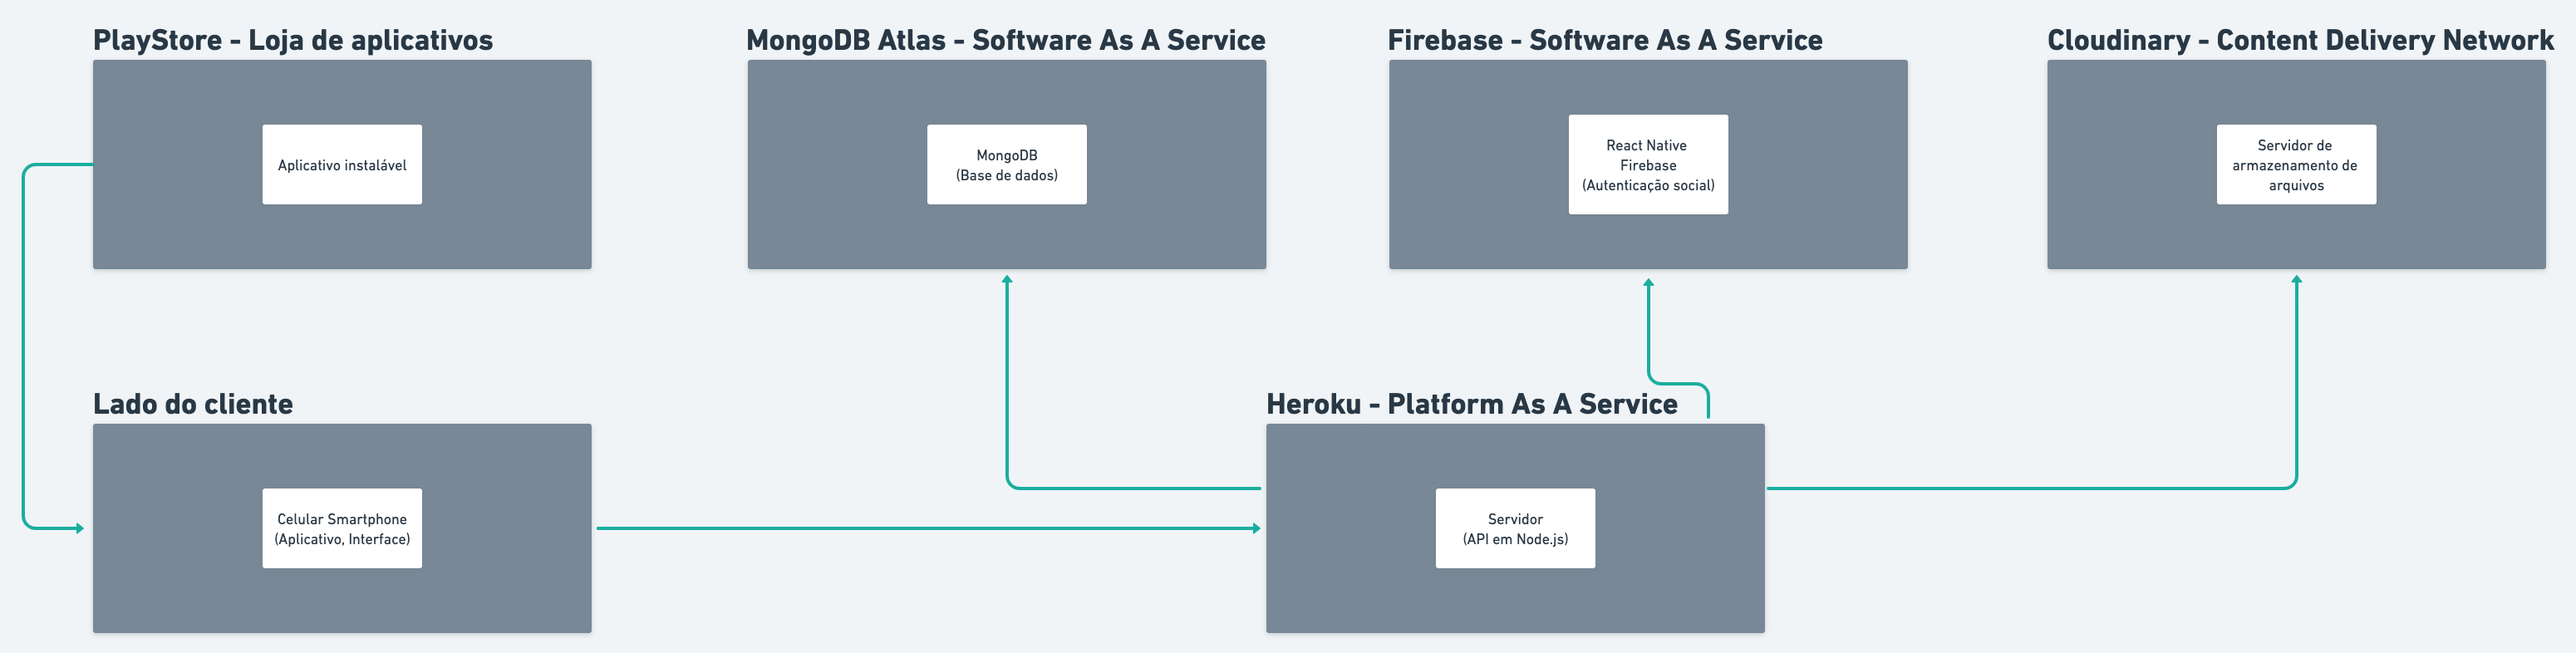
\includegraphics[width=0.9\textwidth]{anexos/arquitetura.png}

	\end{figure}


\subsection{Arquitetura de comunicação}

\pagebreak

\section{Definição do escopo a ser desenvolvido}
\subsection{Entregáveis de modelagem}
\begin{itemize}
    \item Levantamento de requisitos
    
    A análise de requisitos do nosso aplicativo está relacionada com as funcionalidades do sistema e com as prioridades diretamente ligadas à ele. Abaixo, eles estão divididos com suas respectivas funções que englobam tantos os requisitos funcionais, ou seja, declaração dos comportamentos que o sistema deve ter e os requisitos não funcionais que são as restrições colocadas sobre como o sistema deve realizar seus requisitos.
    A seguir as tabelas com os levantamentos dos requisitos funcionais e não funcionais:

\begin{quadro}[htb]
\centering
\ABNTEXfontereduzida
\caption[Requisitos Funcionais]{Requisitos Funcionais}
\label{quadro-exemplo}
\begin{tabular}{|p{4.0cm}|p{4.0cm}|p{4.0cm}|}
  \hline
   \thead{Código} & \thead{Requisito}  & \thead{Descrição} \\
    \hline
    RF01 & Permitir consultar notícias relacionadas a pessoas neuro divergentes.  & Mostra as notícias dentro da aba news.
Mostrar a imagem, título e início do texto que estão associados a notícia 
Para cada notícia listada dentro da aba news, vai ser possível ter a opção de ir para um navegador externo ou continuar no app.\\
    \hline
    RF02 & Permitir criar, editar e excluir subcategorias de discussões dos fóruns criados pelo próprio usuário. &
    O usuário consegue criar uma nova subcategoria dentro de uma categoria 
O usuário que criou a subcategoria consegue editar o título das categorias criadas. 
O usuário consegue excluir a categoria que foi criada, recebendo um aviso se realmente é aquilo que ele deseja fazer. 
\\
   \hline
   RF03 & Permitir criar, editar e excluir posts de discussões que foram criados pelos próprio usuário.  & O usuário consegue criar no novo post em dentro de uma subcategoria. 
O usuário consegue editar um novo post dentro de uma subcategoria. 
O usuário consegue excluir um post dentro de uma subcategoria.\\
    \hline
   RF04 & Postar comentários dentro das subcategorias de discussões dos fóruns criados. & Ter um caixa de texto com um limite caracteres para o comentário ser postado.
Cada postagem precisa mostrar o usuário, data no formato DD/MM/AAAA.
Mostrar toda a mensagem, sem a necessidade de clicar em ver mais.\\
    \hline
   RF05 & Compartilhar imagem dentro das postagens de subcategorias dos fóruns criados. &
    Toda nova postagem vai ser necessário também ter um lugar para fazer o upload de uma imagem para ser postada.  \\
    \hline
   RF06 & Compartilhar nos aplicativos compatíveis as notícias e os posts das subcategorias de discussões dos fóruns criados.  & Apresentar uma lugar para que consiga compartilhar o post.
Os posts precisam ser compartilhados com os aplicativos compatíveis.\\
    \hline
   RF07 & Favoritar mensagens dentro das subcategorias de discussões dos fóruns criados. & Deixar favoritar as mensagens. \\
    \hline
   RF08 & Adicionar, editar e excluir uma avaliação na seção 'Locais Avaliados'. & Fazer o cadastro de um local.
Todas as informações cadastradas podem ser editadas.
\\
\hline
\end{tabular}
\end{quadro}

\begin{quadro}[htb]
\centering
\ABNTEXfontereduzida
\caption[Requisitos Funcionais]{Requisitos Funcionais}
\label{quadro-exemplo}
\begin{tabular}{|p{4.0cm}|p{4.0cm}|p{4.0cm}|}
  \hline
   \thead{Código} & \thead{Requisito}  & \thead{Descrição} \\
    \hline
    RF09 & Permitir consultar notícias relacionadas a pessoas neuro divergentes.  & Mostra as notícias dentro da aba news. Mostrar a imagem, título e início do texto que estão associados a notícia.Para cada notícia listada dentro da aba news, vai ser possível ter a opção de ir para um navegador externo ou continuar no app.\\
    \hline
    RF10 & Permitir criar, editar e excluir subcategorias de discussões dos fóruns criados pelo próprio usuário. &
    O usuário consegue criar uma nova subcategoria dentro de uma categoria. O usuário que criou a subcategoria consegue editar o título das categorias criadas. O usuário consegue excluir a categoria que foi criada, recebendo um aviso se realmente é aquilo que ele deseja fazer. 
\\
   \hline
   RF11 & Permitir criar, editar e excluir posts de discussões que foram criados pelos próprio usuário.  & O usuário consegue criar no novo post em dentro de uma subcategoria. 
O usuário consegue editar um novo post dentro de uma subcategoria. O usuário consegue excluir um post dentro de uma subcategoria.\\
    \hline
   RF12 & Postar comentários dentro das subcategorias de discussões dos fóruns criados. & Ter um caixa de texto com um limite caracteres para o comentário ser postado. Cada postagem precisa mostrar o usuário, data no formato DD/MM/AAAA. Mostrar toda a mensagem, sem a necessidade de clicar em ver mais.\\
    \hline
   RF13 & Compartilhar imagem dentro das postagens de subcategorias dos fóruns criados. &
    Toda nova postagem vai ser necessário também ter um lugar para fazer o upload de uma imagem para ser postada.  \\
    \hline
   RF14 & Compartilhar nos aplicativos compatíveis as notícias e os posts das subcategorias de discussões dos fóruns criados.  & Apresentar uma lugar para que consiga compartilhar o post.
Os posts precisam ser compartilhados com os aplicativos compatíveis.\\
    \hline
   RF15 & Favoritar mensagens dentro das subcategorias de discussões dos fóruns criados. & Deixar favoritar as mensagens. \\
    \hline
\end{tabular}
\end{quadro}

    
\begin{quadro}[htb]
\centering
\ABNTEXfontereduzida
\caption[Requisitos Não Funcionais]{Requisitos Não Funcionais}
\label{quadro-exemplo}
\begin{tabular}{|p{4.0cm}|p{4.0cm}|p{4.0cm}|}
  \hline
   \thead{Código} & \thead{Categoria}  & \thead{Requisito} \\
    \hline
    RNF01 & Portabilidade &
    Deve ter compatibilidade com o sistema operacional Android.\\
   \hline
    RNF02 & Confiabilidade & O sistema deve estar disponível 24 horas por dia,7 dias por semana, com tolerância de 0,1\% de falhas. \\
    \hline
   RNF03 & Desempenho & O sistema deve responder em, no máximo, 0,4 segundos a todas as requisições enviadas para o servidor. \\
    \hline
   RNF04 & Desempenho & Os servidores devem estar sempre online para que o aplicativo funcione corretamente. \\
    \hline
   RNF05 & Desempenho & Para facilitar a visualização dos LOGS deve haver a data contendo o dia, mês, ano, hora e minutos e uma legenda.\\
    \hline
\end{tabular}
\end{quadro}
\end{itemize}

\begin{itemize}
\item Regras de Negócio

Recomenda-se atenção especial para as seguintes regras de negócio descrito no quadro 5:
\begin{quadro}[htb]
\centering
\ABNTEXfontereduzida
\caption[Regras de Negócio]{Regras de Negócio}
\label{quadro-exemplo}
\begin{tabular}{|p{6.3cm}|p{6.3cm}|}
  \hline
   \thead{Código} & \thead{Regra de negócio} \\
    \hline
    RN01 & É obrigatório que o usuário tenha uma conta Google para fazer o login na plataforma. \\
   \hline
    RN02 & Somente após finalizado o cadastro contendo todas as informações obrigatórias (login social, neuro interesse e motivação) o usuário obterá acesso à plataforma.\\
    \hline
   RN03 & Caso o usuário seja o criador de uma subcategoria, será possível editá-la e excluí-la.  \\
    \hline
   RN04 & Somente o usuário que é criador de uma avaliação da seção ‘Locais Avaliados’ é capaz de editá-la ou excluí-la. \\
    \hline
   RN05 & O recebimento de mensagens requer a permissão do usuário. \\
    \hline
   RN06 & Não devem haver subcategorias com o mesmo nome. \\
    \hline
   RN07 & Deverão ser mostradas de forma ranqueada as categorias, subcategorias e posts mais relevantes.\\
    \hline
   RN08 & É obrigatório que os posts publicados contenham título e texto.\\
    \hline
   RN09 & Caso o post seja editado, deve ser explicitado.\\
    \hline
\end{tabular}
\end{quadro}


\end{itemize}

\chapter{Casos de Uso}
Os casos de uso a seguir representam uma possível utilização do nosso sistema por ator, seja ele o usuário ou administrador.

\nopagebreak

\section{UC01: Fazer Login}

\subsection{Atores:}
Cliente
\subsection{Descrição:}
Ao realizar o processo de login, o usuário terá acesso a todas as funcionalidades do aplicativo como consultar o feed de notícias, ter acesso ao fórum podendo criar subcategorias e post e compartilhar informações nos canais de texto, enviar mensagens privadas a outras pessoas que também estão logadas no app e avaliar locais a partir da sua vivência deste estabelecimento.
\subsection{Fluxo de eventos:}
Fluxo Básico:
\begin{itemize}
    \item O usuário entra no aplicativo e visualiza a tela de login;
    \item O usuário insere seu email e senha;
    \item Usuário entra no aplicativo;
    \item O caso de uso é encerrado. 
\end{itemize}

\subsection{Fluxos alternativos:}
O usuário esqueceu a senha:
\begin{itemize}
    \item O usuário entra no aplicativo e visualiza a tela de login;
    \item O usuário insere seu email e senha;
    \item O sistema informa que a senha inserida está incorreta.
    \item O usuário clica em "Esqueci minha senha";
    \item O sistema envia um e-mail para o ator para trocar a senha;
    \item O usuário abre o e-mail e redefine sua senha;
    \item O fluxo principal é recomeçado. 
    \item O caso de uso é encerrado. 
\end{itemize}
 Preenchimento incorreto da senha:
 \begin{itemize}
     \item O usuário entra no aplicativo e visualiza a tela de login;
     \item O usuário insere seu email e senha;
     \item O sistema informa que a senha inserida está incorreta.
     \item O sistema informa que a senha inserida está incorreta.
     \item O caso de uso é encerrado. 
 \end{itemize}
 Primeiro Acesso
 \begin{itemize}
     \item O usuário entra no aplicativo e visualiza a tela de login;
     \item O usuário clica em "cadastrar";
     \item O sistema apresenta a tela de boas vindas;
     \item O usuário clica em "Avançar"
     \item O usuário insere as informações necessárias para o cadastramento no aplicativo;
     \item O usuário recebe a mensagem de "Cadastro feito com sucesso";
     \item O fluxo principal é começado para o usuário;
     \item O caso de uso é encerrado.
 \end{itemize}
 Login Social (Google): 
\begin{itemize}
    \item O usuário entra no aplicativo e visualiza a tela de login;
    \item O usuário clica no botão de realizar o login social;
    \item O sistema direciona o usuário para link do login social;
    \item O usuário faz sua autenticação com o email social e senha;
    \item O usuário retorna para tela do aplicativo já sendo direcionado para o fluxo principal do app;
    \item O caso de uso é encerrado. 
\end{itemize}
\subsection{Pré-condições}
\begin{itemize}
    \item Ter o aplicativo instalado do aparelho do Cliente;
    \item Ter acesso a internet;
    \item Possuir cadastro/conta no Google. 
\end{itemize}

\subsection{Pós-condições}
Acesso a homepage do aplicativo e de todas as funcionalidades existentes no sistema. 

\section{UC02: Efetuar Cadastro}

\subsection{Atores:}
Visitante;
\subsection{Descrição:}
Esse caso terá como funcionalidade o cadastrar novos usuários na aplicação. 
\subsection{Fluxo de eventos:}
Fluxo Básico: 
\begin{itemize}
    \item O usuário entra no aplicativo e visualiza a tela de login;
    \item O usuário clica em "cadastrar";
    \item O sistema apresenta a tela de boas vindas;
    \item O usuário clica em "Avançar";
    \item O usuário clica em "Cadastrar no App";
    \item O usuário insere as informações necessárias para o cadastramento no aplicativo;
    \item O usuário recebe a mensagem de "Cadastro feito com sucesso";
    \item O fluxo principal é começado para o usuário;
    \item O caso de uso é encerrado.
\end{itemize}

\subsection{Fluxos alternativos:}
Cadastro com a conta Google:
\begin{itemize}
    \item O usuário entra no aplicativo e visualiza a tela de login;
    \item O usuário clica em "cadastrar";
    \item O sistema apresenta a tela de boas vindas;
    \item O usuário clica em "Avançar";
    \item O usuário clica em "Cadastrar com o Google";
    \item O sistema irá direcioná-lo para sua conta google para permitir acesso;
    \item O usuário é retornado para o aplicativo e recebe a mensagem de "Cadastro feito com sucesso";
    \item  O fluxo principal é começado para o usuário;
    \item O caso de uso é encerrado.
\end{itemize}
\subsection{Pré-condições}
\begin{itemize}
    \item Ter o aplicativo instalado do aparelho do Cliente;
    \item Ter acesso a internet;
\end{itemize}

\subsection{Pós-condições}
O Visitante vai se tornar um novo usuário da aplicação.
\section{UC03: Editar perfil}

\subsection{Atores:}
Cliente;
\subsection{Descrição:}
Esse caso de uso ocorre quando o usuário logado no aplicativo deseja alterar suas informações de perfil. 

\subsection{Fluxo Básico: }
\begin{itemize}
    \item O usuário seleciona a seção "Perfil";
    \item O usuário seleciona "Editar Perfil";
    \item O sistema exibe as categorias do perfil: nome, data de nascimento, e-mail, neuro diversidades que tem interesse, abertura de mensagens privadas;
    \item O usuário seleciona a(s) categoria(s) que deseja editar;
    \item O usuário atualiza as suas informações e pressiona no botão "Salvar";
    \item O sistema valida os dados conforme requeridos e atualiza o perfil do assinante. 
    \item O caso de uso é encerrado. 
\end{itemize}

\subsection{Pré-condições}
O usuário deve estar logado no aplicativo. 
\subsection{Pós-condições}
Ao final das alterações feitas pelo usuário, a seção perfil deve estar atualizada. 

\section{UC04: Consultar mensagens no Fórum}

\subsection{Atores:}
Clente
\subsection{Descrição:}
O cliente deve encontrar todas as mensagens ocorridas dentro das subcategorias.
\subsection{Fluxo Básico:}
\begin{itemize}
    \item O usuário seleciona a seção "Fórum";
    \item O usuário seleciona a categoria desejada;
    \item O sistema mostra todas as subcategorias relacionadas categoria escolhida pelo usuário;
    \item O usuário escolhe uma subcategoria;
    \item O sistema mostra todas as mensagens ocorridas nesse canal de texto até o momento. 
    \item O caso de uso é encerrado.
\end{itemize}

\subsection{Pré-condições}
O usuário deve estar logado no aplicativo. 
\subsection{Pós-condições}
Ao final da escolha da subcategoria, deverá mostrar todas as mensagens do canal de texto. 
\section{UC05: Remover mensagens no Fórum}

\subsection{Atores:}
Administrador, Cliente;
\subsection{Descrição:}
Ao criar uma subcategoria, o cliente poderá excluir sua própria mensagem dentro do canal de texto e poderá excluir as mensagens de outros dentro dessa subcategoria que ele criou. O Administrador terá permissão de excluir as mensagens das subcategorias, até mesmo do criador dela.
\subsection{Fluxo Básico: }
Para o cliente:
\begin{itemize}
    \item O usuário seleciona a seção "Fórum";
    \item O usuário seleciona a categoria desejada;
    \item O sistema mostra todas as subcategorias relacionadas à categoria escolhida pelo usuário;
    \item O usuário escolhe uma subcategoria;
    \item O sistema mostra todas as mensagens ocorridas nesse canal de texto até o momento. 
    \item O usuário seleciona a mensagem que deseja excluir;
    \item O sistema atualiza o canal de texto retirando a mensagem excluída. 
    \item O  caso de uso é encerrado. 
\end{itemize}
Para o Administrador:
\begin{itemize}
    \item O administrador seleciona a seção "Fórum";
    \item O administrador seleciona a categoria desejada;
    \item O administrador mostra todas as subcategorias relacionadas à categoria escolhida pelo usuário;
    \item O administrador escolhe uma subcategoria;
    \item O sistema mostra todas as mensagens ocorridas nesse canal de texto até o momento. 
    \item O administrador seleciona a mensagem que deseja excluir;
    \item O sistema atualiza o canal de texto retirando a mensagem excluída. 
    \item O caso de uso é encerrado. 
\end{itemize}

\subsection{Pré-condições}
Para o Cliente: 
\begin{itemize}
    \item O usuário deve estar logado no aplicativo e ser o criador do canal de texto
\end{itemize}
Para o Administrador:
\begin{itemize}
    \item O administrador deve ter a chave de permissão. 
\end{itemize}
\subsection{Pós-condições}
O sistema deve atualizar o canal de texto já retirando a mensagem de texto excluída. 
\section{UC06: Curtir mensagens no Fórum}

\subsection{Atores:}
Cliente;
\subsection{Descrição:}
O usuário poderá curtir uma mensagem de texto dentro das subcategorias;
\subsection{Fluxo Básico:}
\begin{itemize}
    \item O usuário seleciona a seção "Fórum";
    \item O usuário seleciona a categoria desejada;
    \item O sistema mostra todas as subcategorias relacionadas à categoria escolhida pelo usuário;
    \item O usuário escolhe uma subcategoria;
    \item O sistema mostra todas as mensagens ocorridas nesse canal de texto até o momento. 
    \item O usuário seleciona a mensagem desejada e clica em "curtir mensagem";
    \item O sistema atualiza o canal de texto; 
    \item O caso de uso é encerrado. 
\end{itemize}
\subsection{Pré-condições}
O cliente deve estar logado no aplicativo.
\subsection{Pós-condições}
O sistema irá atualizar o número de curtidas da mensagem selecionada pelo usuário. 
\section{UC07: Criar categoria}

\subsection{Atores:}
Administrador.

\subsection{Descrição:}
O Administrador tem permissão de criar uma categoria dentro do fórum. 
\subsection{Fluxo Básico:}

\begin{itemize}
    \item O administrador seleciona a seção "Fórum";
    \item O administrador seleciona o botão "+";
    \item O sistema irá apresentar a opção "Criar uma Categoria";
    \item Ao clicar em criar uma categoria, o administrador deverá escrever o nome da categoria e clicar em "Criar canal de texto";
    \item O sistema atualizará com a nova categoria criada. 
    \item O caso de uso é encerrado. 
\end{itemize}

\subsection{Pré-condições}
O administrador deve ter a chave de permissão;
\subsection{Pós-condições}
O sistema mostrará a nova categoria criada pelo administrador e deve permitir que a partir dessa categoria sejam criadas subcategorias pelos usuários e administradores. 
\section{UC08: Criar uma subcategoria}

\subsection{Atores:}
 Administrador, Cliente.
\subsection{Descrição:}
O cliente e/ou administrador devem conseguir criar subcategorias a partir das categorias já criadas pelo administrador.
\subsection{Fluxo Básico para o Cliente e/ou Administrador: }

\begin{itemize}
    \item O usuário seleciona a seção "Fórum";
    \item O usuário seleciona a categoria desejada;
    \item O usuário clica no botão "+" ao lado do nome da categoria selecionada;
    \item O usuário escreve o nome da subcategoria e clica em "Salvar"
    \item O sistema atualiza com a nova subcategoria criada. 
    \item O caso de uso é encerrado. 
\end{itemize}

\subsection{Pré-condições}
O cliente deve estar logado no app e o administrador deve ter a chave de permissão;
\subsection{Pós-condições}
O sistema mostrará a nova categoria criada pelo administrador ou usuário. 
\section{UC09: Remover uma subcategoria}

\subsection{Atores:}
Administrador, Cliente.
\subsection{Descrição:}
O cliente e/ou administrador devem conseguir remover uma subcategoria. 
\subsection{Fluxo Básico para o cliente:}

\begin{itemize}
    \item O usuário seleciona a seção "Fórum";
    \item O usuário seleciona uma categoria;
    \item O sistema mostra todas as subcategoria existentes;
    \item O cliente seleciona a subcategoria desejada;
    \item O cliente pressiona a subcategoria;
    \item Caso o cliente seja o criador dessa subcategoria, o sistema irá mostrar uma pop-up perguntando para o usuário se ele deseja excluir a subcategoria criada. 
    \item O usuário clica em "Sim";
    \item O sistema exclui a subcategoria;
    \item O caso de uso é encerrado. 
\end{itemize}
\subsection{Fluxo de Excessão:}
Fluxo básico para o administrador
\begin{itemize}
    \item O administrador seleciona a seção "Fórum";
    \item O administrador seleciona uma categoria;
    \item O sistema mostra todas as subcategoria existentes;
    \item O administrador seleciona a subcategoria desejada;
    \item O administrador pressiona a subcategoria;
    \item O sistema irá mostrar uma pop-up perguntando para o administrador se ele deseja excluir a subcategoria pressionada;
    \item O administrador clica em "Sim";
    \item O sistema exclui a subcategoria;
    \item O caso de uso é encerrado. 
\end{itemize}
\subsection{Pré-condições}
Para o cliente
\begin{itemize}
    \item O cliente deve estar logado no app e ser o criador do subcategoria escolhida. 
\end{itemize}
Para o Administrador
\begin{itemize}
    \item O administrador deve ter a chave de permissão;
\end{itemize}
\subsection{Pós-condições}
O sistema irá atualizar removendo a subcategoria selecionada. 
\section{UC10: Criação do Local Avaliado}

\subsection{Atores:}
Cliente
\subsection{Descrição:}
O usuário poderá avaliar positivamente ou negativamente os estabelecimentos que ele queira recomendar para outras pessoas dentro da rede social. 
\subsection{Fluxo Básico:}

\begin{itemize}
    \item O usuário clica na seção 'Locais Avaliados';
    \item O usuário clica na aba 'Meus Locais Avaliados';
    \item O usuário clica em "Adicionar Avaliação";
    \item O sistema fornece a parte de "Adicionar Avaliação";
    \item O usuário cadastra a avaliação e clica em "Salvar";
    \item O sistema busca identificar e confirmar os dados inseridos pelo usuário.
    \item O sistema retorna "Avaliação Adicionada" e adiciona na lista de locais avaliados;
    \item O caso de uso é encerrado.
\end{itemize}
\subsection{Fluxo de Excessão:}
O usuário não insere todos os dados necessários: 
\begin{itemize}
    \item O usuário clica na aba 'Meus Locais Avaliados';
    \item O usuário clica em "Adicionar Avaliação";
    \item O sistema fornece a parte de "Adicionar Avaliação";
    \item O usuário cadastra a avaliação e clica em "Salvar";
    \item O sistema retorna os dados obrigatórios que o usuário não inseriu ao cadastrar e impede que a avaliação seja salva;
    \item O caso de uso é encerrado. 
\end{itemize}
\subsection{Pré-condições}
\begin{itemize}
    \item Estar logado no aplicativo;
    \item Usuário com acesso a internet. 
\end{itemize}
\subsection{Pós-condições}
Apresentar o Local Avaliado cadastrado pelo usuário na aba 'Locais Avaliados'. 
\section{UC11: Consultar Locais Avaliados}

\subsection{Atores:}
Cliente;
\subsection{Descrição:}
Consultar todos os locais avaliados já adicionados pelos usuários. 
\subsection{Fluxo Básico:}

\begin{itemize}
    \item O usuário clica na seção 'Locais Avaliados';
    \item O usuário clica na aba 'Todos Locais Avaliados';  
    \item O usuário clica no nome de um local avaliado;
    \item O usuário visualiza a avaliação;
    \item O caso de uso é encerrado. 
\end{itemize}

\subsection{Pré-condições}
\begin{itemize}
    \item Estar logado no aplicativo;
    \item Usuário com acesso a internet. 
\end{itemize}
\subsection{Pós-condições}
\begin{itemize}
    \item Apresentar todos os locais avaliados já cadastrados no aplicativo;
    \item Apresentar as informações do local avaliado quando o usuário clica no nome do local avaliado na qual ele quer consultar. 
\end{itemize}

\section{UC12: Editar Locais Avaliados}

\subsection{Atores:}
Cliente. 
\subsection{Descrição:}
O usuário poderá editar as informações inseridas por ele na aba de 'Meus Locais Avaliados'.
\subsection{Fluxo Básico:}

\begin{itemize}
    \item O usuário clica na seção 'Locais Avaliados';
    \item O usuário clica na aba 'Meus Locais Avaliados';
    \item O usuário pressiona o local avaliado na qual ele quer editar;
    \item O sistema mostra uma pop-up com a opção "Editar Local Avaliado";
    \item O usuário clica em "Editar Local Avaliado";
    \item O usuário edita as informações e clica em "Salvar";
    \item O sistema confirmar os dados inseridos pelo usuário;
    \item O caso de uso é encerrado. 
\end{itemize}

\subsection{Pré-condições}
\begin{itemize}
    \item Estar logado no aplicativo;
    \item Usuário com acesso a internet. 
    \item Ser o criador do local avaliado. 
\end{itemize}

\subsection{Pós-condições}
O sistema deve apresentar o local avaliado com as novas informações inseridas pelo usuário.

\section{UC13: Remover Local Avaliado}

\subsection{Atores:}
Cliente.
\subsection{Descrição:}
O usuário poderá excluir o local avaliado inserido por ele na aba de 'Meus Locais Avaliados'.
\subsection{Fluxo Básico:}

\begin{itemize}
    \item O usuário clica na seção 'Locais Avaliados';
    \item O usuário clica na aba 'Meus Locais Avaliados';
    \item O usuário pressiona o local avaliado na qual ele quer excluir;
    \item O sistema mostra uma pop-up com a opção "Excluir Local Avaliado"; 
    \item O usuário clica em "Excluir Local Avaliado";
    \item O usuário exclui local avaliado";
    \item O sistema atualiza e retorna com a mensagem "local excluído com sucesso";
    \item O caso de uso é encerrado. 
\end{itemize}
\subsection{Pré-condições}
\begin{itemize}
    \item Estar logado no aplicativo;
    \item Usuário com acesso a internet. 
    \item Ser o criador do local avaliado. 
\end{itemize}

\subsection{Pós-condições}
O sistema deve excluir o local avaliado escolhido pelo usuário da lista "Meus Locais Avaliados" e "Todos os Locais Avalaidos".

\section{UC14: Visualizar Perfil dos usuários}

\subsection{Atores:}
Cliente. 
\subsection{Descrição:}
Visualiza perfil do cliente quando clica na foto de perfil ou no nome do usuário.
\subsection{Fluxo Básico:}

\begin{itemize}
    \item O usuário clica na imagem do usuário;
    \item O usuário visualiza o perfil de outro usuário;
    \item O caso de uso está encerrado.
\end{itemize}
\subsection{Fluxo alternativo:}
\begin{itemize}
    \item O usuário clica no nome do usuário;
    \item O usuário visualiza o perfil de outro usuário;
    \item O caso de uso está encerrado.
\end{itemize}
\subsection{Pré-condições}
\begin{itemize}
    \item Estar logado no aplicativo;
    \item Usuário com acesso a internet. 
\end{itemize}
\subsection{Pós-condições}
 O sistema irá mostrar uma nova tela com todas as informações do usuário escolhido. 
\section{UC15: Troca de mensagens de texto em chat individual}

\subsection{Atores:}
Cliente. 
\subsection{Descrição:}
Nesse caso de uso, o usuário poderá enviar e receber mensagens por meio de um chat privado entre os usuários. 
\subsection{Fluxo Básico:}

\begin{itemize}
    \item O usuário clica na aba "Chat";
    \item O usuário clica em um dos usuários que estão em sua lista;
    \item O usuário envia mensagem;
    \item O caso de uso é encerrado. 
\end{itemize}
\subsection{Fluxo alternativo:}
Primeira vez do usuário enviando mensagem. 
\begin{itemize}
    \item O usuário clica na imagem ou no nome do outro usuário;
    \item O usuário visualiza o perfil desse usuário;
    \item O usuário clica em "Enviar Mensagem";
    \item O sistema abre o chat entre esses dois usuários;
    \item O usuário envia a mensagem;
    \item O caso de uso é encerrado 
\end{itemize}

\subsection{Pré-condições}
\begin{itemize}
    \item  Estar logado no aplicativo;
    \item Usuário com acesso a internet. 
\end{itemize}
\subsection{Pós-condições}
O usuário deve ter sua mensagem entregue e recebida pelo outro usuário. 
\section{UC16: Visualizar notícias}

\subsection{Atores:}
Cliente;
\subsection{Descrição:}
O usuário deverá visualizar todas as notícias dentro da seção "Feed de notícias". 
\subsection{Fluxo Básico:}

\begin{itemize}
    \item O usuário logado entra na seção "Feed de notícias";
    \item O usuário visualiza as notícias;
    \item O caso de uso é encerrado. 
\end{itemize}
\subsection{Fluxo alternativo:}
O usuário clica na notícia para visualizar os detalhes. 
\begin{itemize}
    \item O usuário logado entra na seção "Feed de notícias";
    \item O usuário visualiza as notícias;
    \item O usuário clica em uma notícia;
    \item O sistema leva o usuário para uma nova tela com os detalhamentos da notícia clicada pelo usuário;
    \item O caso de uso é encerrado. 
\end{itemize}
\subsection{Pré-condições}
\begin{itemize}
    \item Estar logado no aplicativo;
    \item Usuário com acesso a internet. 
\end{itemize}

\subsection{Pós-condições}
 O sistema deve mostrar as notícias relacionadas ao tema de crianças neuro diversas. 
\section{UC17: Criar um Post: }

\subsection{Atores:}
Cliente.
\subsection{Descrição:}
O usuário poderá criar um post a partir das subcategorias existentes. 
\subsection{Fluxo Básico:}

\begin{itemize}
    \item O usuário seleciona uma subcategoria selecionada;
    \item O usuário clica no botão "+" ao lado do nome da subcategoria selecionada para criar o post;
    \item O usuário insere as informações necessárias para a criação do post;
    \item O usuário clica em "Criar Post"; 
    \item O caso de uso é encerrado. 
\end{itemize}

\subsection{Pré-condições}
\begin{itemize}
    \item  Estar logado no aplicativo;
    \item Usuário com acesso a internet. 
\end{itemize}

\subsection{Pós-condições}
O sistema deve permitir a criação do post feita pelo usuário. 
\section{UC18: Remover um Post:  }

\subsection{Atores:}
 Administrador, Cliente. 
\subsection{Descrição:}
O usuário poderá remover um post a partir das subcategorias existentes. 
\subsection{Fluxo Básico::}

\begin{itemize}
    \item O usuário seleciona um post;
    \item O usuário clica na opção "Apagar Post";
    \item O sistema apaga o post criado pelo usuário;
    \item O caso de uso é encerrado.
\end{itemize}
\subsection{Fluxos alternativos:}
O administrador remove um post
\begin{itemize}
    \item O administrador seleciona um post;
    \item O administrador clica na opção "Apagar Post";
    \item O sistema apaga o post criado pelo administrador;
    \item O caso de uso é encerrado. 
\end{itemize}
\subsection{Pré-condições}
\begin{itemize}
    \item Estar logado no aplicativo;
    \item Usuário com acesso a internet. 
    \item O usuário deve ser o criado do post criado
\end{itemize}
\subsection{Pós-condições}
O sistema deve atualizar com o post excluído pelo usuário.  
\section{UC19: Comentar Post: }

\subsection{Atores:}
 Cliente. 
\subsection{Descrição:}
  O usuário poderá comentar um post a partir das subcategorias existentes. 
\subsection{Fluxo Básico:}

\begin{itemize}
    \item O usuário seleciona um post;
    \item O usuário clica na opção "Comentar";
    \item O usuário adiciona um comentário no post seleciona;
    \item O caso de uso é encerrado. 
\end{itemize}

\subsection{Pré-condições}
\begin{itemize}
    \item Estar logado no aplicativo;
    \item Usuário com acesso a internet. 
\end{itemize}
\subsection{Pós-condições}
O sistema deve mostrar o comentário do usuário no post selecionado.   

\section{UC20: Curtir Post: }

\subsection{Atores:}
 Cliente. 
\subsection{Descrição:}
O usuário poderá curtir um post criado na subcategoria.
\subsection{Fluxo Básico:}

\begin{itemize}
    \item O usuário seleciona um post;
    \item O usuário clica em "Curtir";
    \item O caso de uso é encerrado.
\end{itemize}

\subsection{Pré-condições}
\begin{itemize}
    \item Estar logado no aplicativo;
    \item Usuário com acesso a internet. 
\end{itemize}

\subsection{Pós-condições}
O sistema deve atualizar as curtidas realizadas no post do usuário. 
\section{UC21: Comentar notícias: }

\subsection{Atores:}
Cliente;
\subsection{Descrição:}
 O usuário deve conseguir comentar uma notícias na seção "Feed de notícias". 
\subsection{Fluxo Básico:}

\begin{itemize}
    \item O usuário logado entra na seção "Feed de notícias";
    \item O usuário visualiza as notícias;
    \item O usuário clica em uma notícia;
    \item O sistema leva o usuário para uma nova tela com os detalhamentos da notícia clicada pelo usuário;
    \item O usuário escreve seu comentário;
    \item O usuário clica em "Comentar";
    \item O caso de uso é encerrado. 
\end{itemize}

\subsection{Pré-condições}
\begin{itemize}
    \item Estar logado no aplicativo;
    \item Usuário com acesso a internet. 
\end{itemize}
\subsection{Pós-condições}
Após o usuário salvar seu comentário, o sistema deve apresentar o comentário realizado pelo usuário; 


\chapter{Diagramas dos Casos de Usos}
\begin{figure}[htb]

    \centering
	\caption{\label{fig_arq_virado}Diagrama de Caso de Uso Login}
	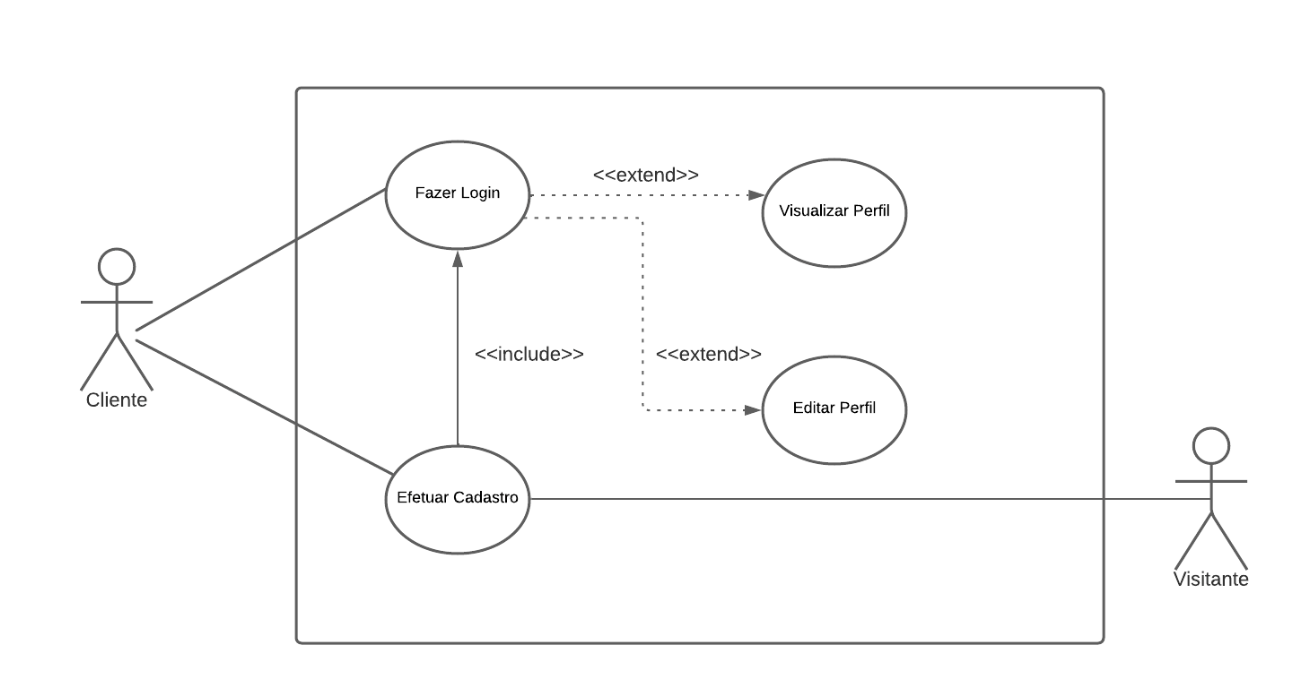
\includegraphics[width=0.9\textwidth]{anexos/diagramaLogin.png}

	\end{figure}
\begin{figure}[htb]

    \centering
	\caption{\label{fig_arq_virado}Diagrama de Caso de Uso Fórum}
	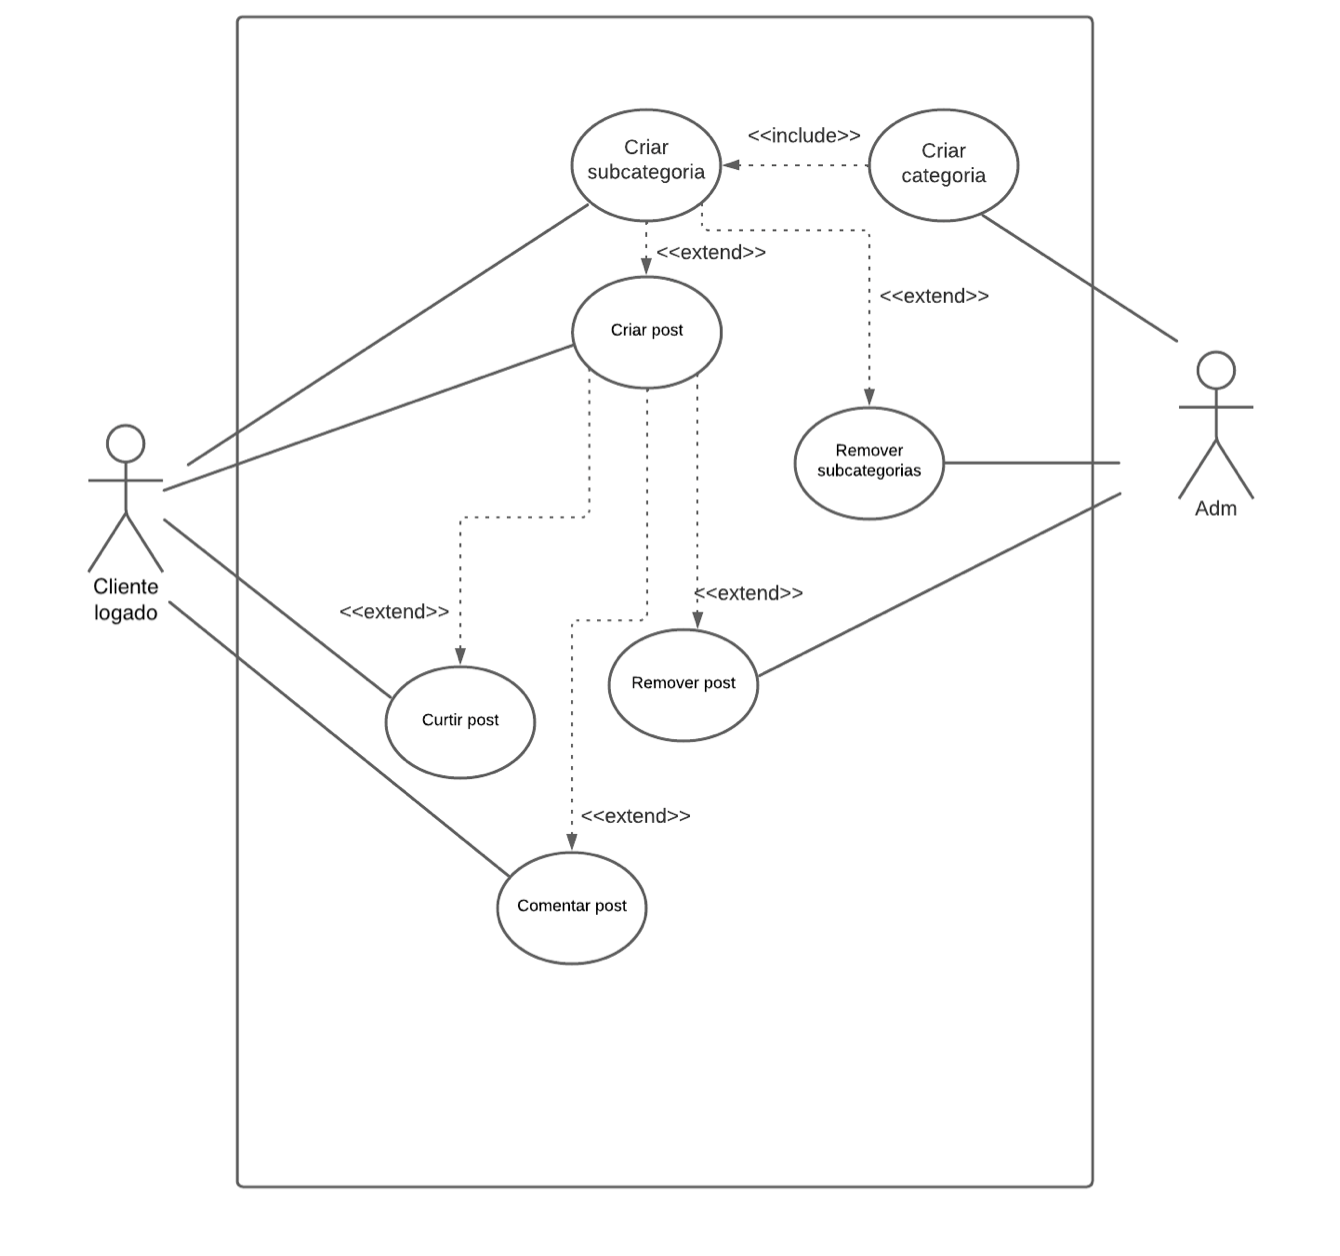
\includegraphics[width=0.9\textwidth]{anexos/diagramaForum.png}

	\end{figure}
\begin{figure}[htb]

    \centering
	\caption{\label{fig_arq_virado}Diagrama de Caso de Uso Local Avaliado}
	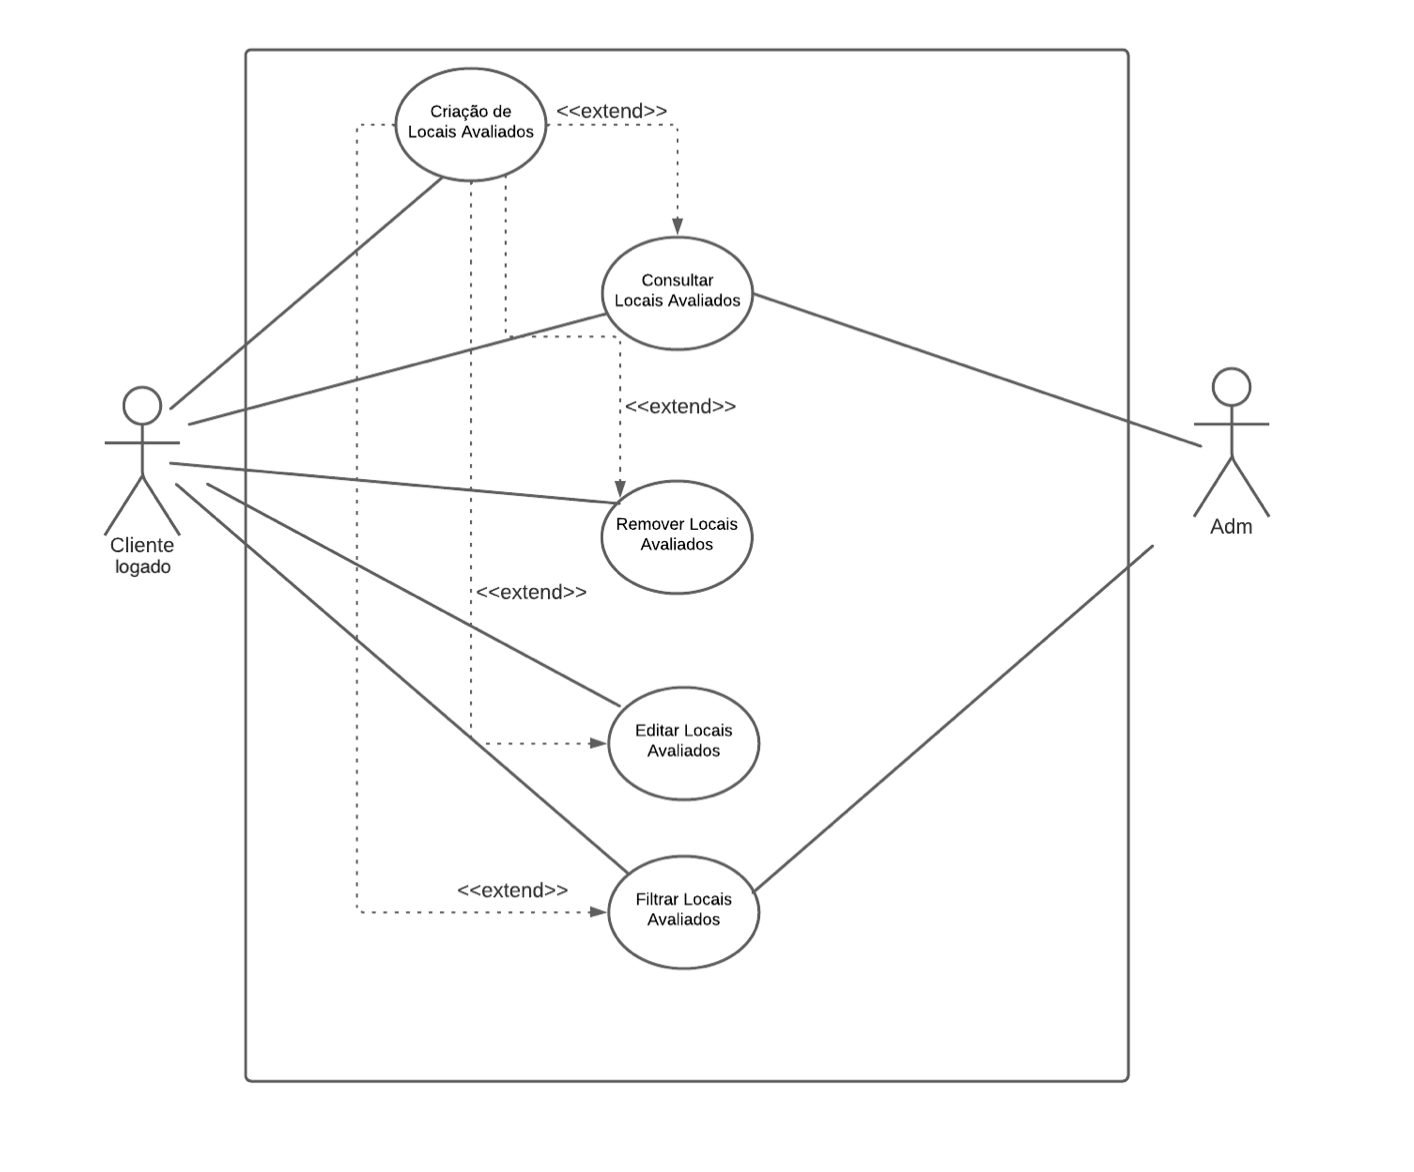
\includegraphics[width=0.9\textwidth]{anexos/diagramaAvaliado.png}

	\end{figure}
\begin{figure}[htb]

    \centering
	\caption{\label{fig_arq_virado}Diagrama de Caso de Uso Troca de Mensagens de Texto}
	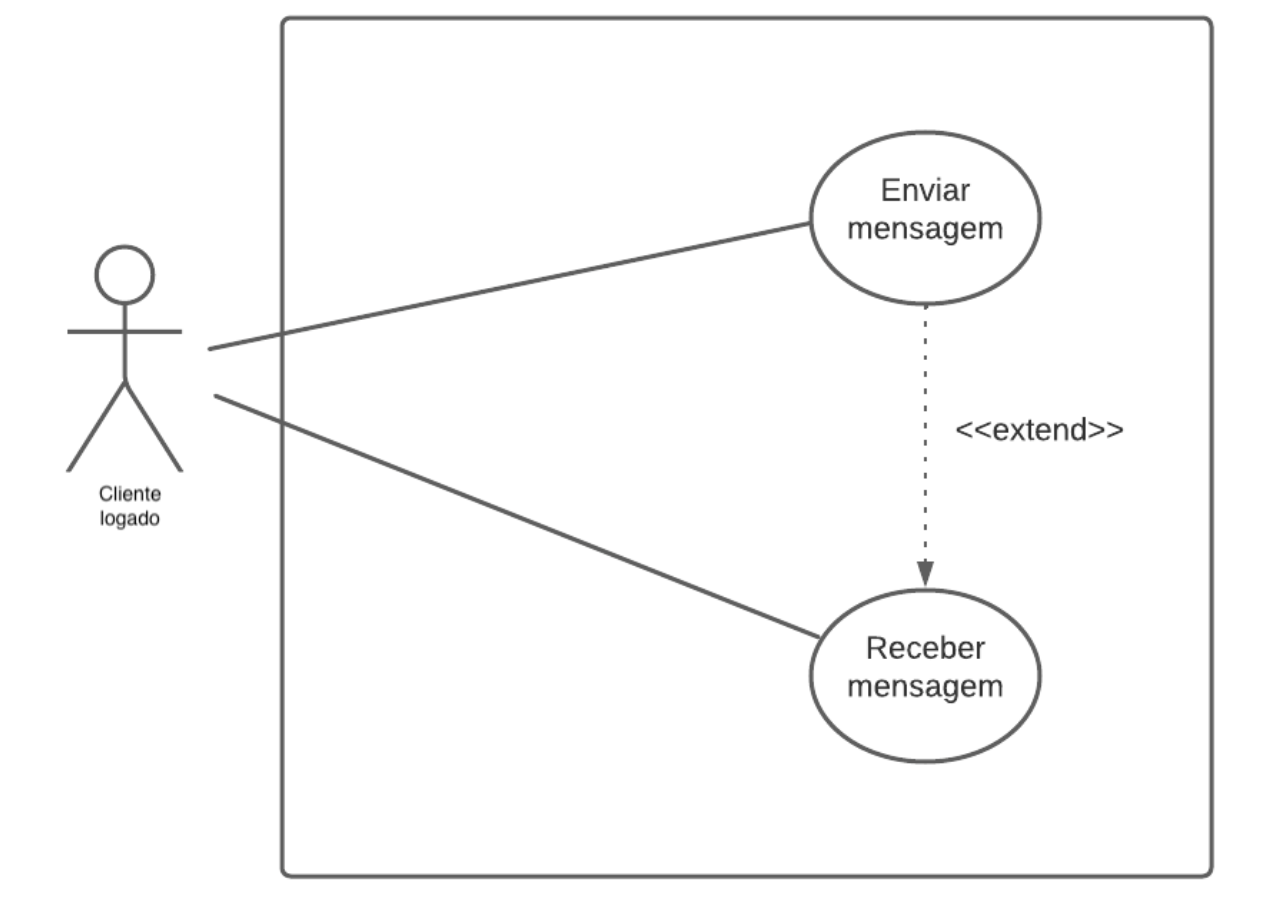
\includegraphics[width=0.9\textwidth]{anexos/diagramaMensagem.png}

	\end{figure}
\begin{figure}[htb]

    \centering
	\caption{\label{fig_arq_virado}Diagrama de Caso de Uso Feed de notícias}
	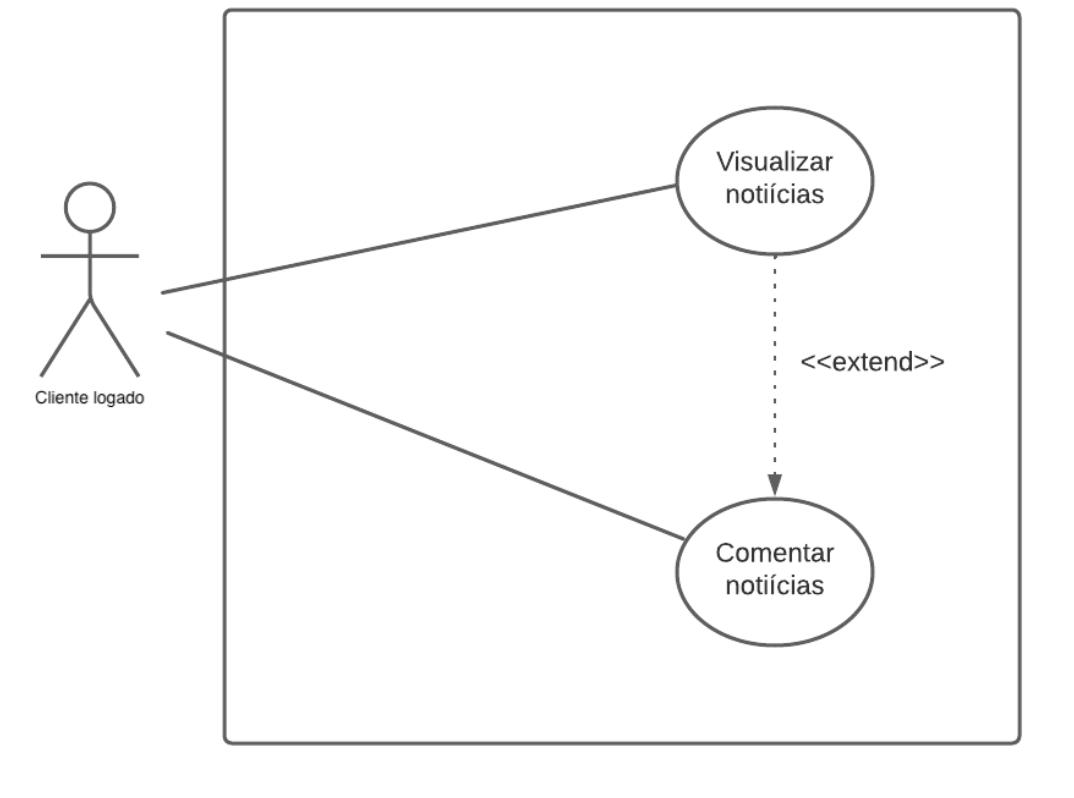
\includegraphics[width=0.9\textwidth]{anexos/diagramaFeed.png}

	\end{figure}



\chapter{Viabilidade Financeira}

% ---

% ---
Neste tópico serão considerados os custos das ferramentas pagas cujo o uso já está previsto no desenvolvimento da aplicação. 

Como ferramentas pagas imprescindíveis para o funcionamento da aplicação prevê-se:

\begin{quadro}[htb]
\centering
\ABNTEXfontereduzida
\caption[Custo das ferramentas]{Custo das ferramentas}
\label{quadro-exemplo}
\begin{tabular}{|p{4.0cm}|p{4.0cm}|p{3.0cm}|}
  \hline
   \thead{Ferramenta} & \thead{Uso}  & \thead{Custo mensal\\(em dólares)} \\
    \hline
    Heroku & API e Banco de dados  & 25,00  \\
    \hline
    Cloudinary & Servidor de arquivos &
    89,00 \\
    \hline
    Firebase & Infraestrutura da aplicação & 5,00  \\
   \hline
\end{tabular}
\end{quadro}

Para o recurso de envio e recebimento de e-mails estão sendo estudadas duas ferramentas: 

\begin{quadro}[htb]
\centering
\ABNTEXfontereduzida
\caption[Custo das ferramentas de email]{Custo das ferramentas de email}
\label{quadro-exemplo}
\begin{tabular}{|p{4.0cm}|p{4.0cm}|p{3.0cm}|}
  \hline
   \thead{Ferramenta} & \thead{Uso}  & \thead{Custo mensal\\(em dólares)} \\
    \hline
    Mailgun & Envio e recebimento de e-mails  & 35,00  \\
    \hline
    Simple Email Service & Envio e recebimento de e-mails &
    0,10*\\
   \hline
\end{tabular}
\end{quadro}

*O custo de U\$0,10 diz respeito a um volume de até mil e-mails enviados/recebidos pela ferramenta e, considerando o alcance inicial da aplicação, pode-se afirmar que este seria o gasto mensal referente ao recurso durante um considerável período de tempo, e por se tratar de um melhor custo benefício, provavelmente será a ferramenta escolhida. 

Tendo em vista que o aplicativo também terá sua versão mobile, devem ser considerados os custos para a postagem nas lojas virtuais mobile: 

\begin{quadro}[htb]
\centering
\ABNTEXfontereduzida
\caption[Custo das ferramentas de loja]{Custo das ferramentas de loja}
\label{quadro-exemplo}
\begin{tabular}{|p{4.0cm}|p{4.0cm}|p{3.0cm}|}
  \hline
   \thead{Store} & \thead{Custo\\(em dólares)} \\
    \hline
    Play Store & 25,00 \\
    \hline
    Apple Store & 99,00**\\
   \hline
\end{tabular}
\end{quadro}

**O custo de U\$99,00 da Apple Store não é pago uma única vez como o da Play Store, é um custo anual, por essa razão ainda está sendo discutida a postagem ou não postagem na plataforma. 

Dessa forma, pode-se considerar como custo inicial, inserindo a postagem, o valor de U\$139,10 e após a postagem, o custo de mantenimento mensal passa a ser U\$114,10. Em caso de necessidade de alteração da ferramenta de envio e recebimento e-mails, o custo pode ser elevado para os valores de U\$174,00 iniciais e U\$149,00 de mantenimento. 

% ---
